% Created 2022-10-10 Mon 11:18
% Intended LaTeX compiler: pdflatex
\documentclass[presentation,aspectratio=1610]{beamer}
\usepackage[utf8]{inputenc}
\usepackage[T1]{fontenc}
\usepackage{graphicx}
\usepackage{grffile}
\usepackage{longtable}
\usepackage{wrapfig}
\usepackage{rotating}
\usepackage[normalem]{ulem}
\usepackage{amsmath}
\usepackage{textcomp}
\usepackage{amssymb}
\usepackage{capt-of}
\usepackage{hyperref}
\usepackage{khpreamble}
\usepackage{pgfplots}
\usepackage{pdfpages}
\usepackage{circuitikz}
\usepgfplotslibrary{groupplots}
\usetikzlibrary{positioning,circuits.plc.ladder}
\renewcommand*{\not}[1]{\ensuremath{\bar{#1}}}
\renewcommand*{\not}[1]{\ensuremath{\overline{#1}}}
\newcommand*{\coil}[1]{to[short] ++(0.5, 0) node[coordinate] (orig) {} arc [start angle=180, end angle=150,radius=8mm] (orig) arc [start angle=180, end angle=210,radius=8mm] (orig) ++(1cm, 0) node[coordinate] (coilend) {} arc [start angle=0, end angle=30,radius=8mm] (coilend) arc [start angle=0, end angle=-30,radius=8mm] (coilend) to[short] ++(0.5cm, 0) (orig) ++(0.5, 0.8) node {#1}}
\newcommand*{\etimer}[2]{to[short] node[coordinate, pos=1.0] (orig) {} ++(0.5, 0) ++(0, -5mm) rectangle ++(5mm ,10mm)   (orig)  ++(0, -10mm) node[coordinate] (corner1) {} rectangle ++(5mm,5mm) node[coordinate] (corner2) {} (corner1) to (corner2) (orig) ++(0mm,-5mm) to ++(5mm,-5mm) (orig) ++(5mm, 0) to[short] ++(5mm, 0) (orig) ++(2.5mm, 8mm) node {#1} (orig) ++(2.5mm, 0) node{#2}}
\makeatletter
%% Push Button
\pgfcircdeclarebipole{}{\ctikzvalof{bipoles/pushbutton/height 2}}{pushedbutton}{\ctikzvalof{bipoles/pushbutton/height}}{\ctikzvalof{bipoles/pushbutton/width}}{
\pgfsetlinewidth{\pgfkeysvalueof{/tikz/circuitikz/bipoles/thickness}\pgfstartlinewidth}
\pgf@circ@res@temp=-\pgfkeysvalueof{/tikz/circuitikz/nodes width}\pgf@circ@Rlen
\advance\pgf@circ@res@temp by -2\pgfstartlinewidth
\pgfpathmoveto{\pgfpoint{\pgf@circ@res@left}{\pgf@circ@res@temp}}
\pgfpathlineto{\pgfpoint{\pgf@circ@res@right}{\pgf@circ@res@temp}}
\pgfpathmoveto{\pgfpoint{0}{\pgf@circ@res@temp}}
\pgfpathlineto{\pgfpoint{0}{\pgf@circ@res@up}}
\pgfusepath{draw}
\pgftransformshift{\pgfpoint{\pgf@circ@res@left}{0pt}}
\pgfnode{ocirc}{center}{}{}{\pgfusepath{draw}}
\pgftransformshift{\pgfpoint{2\pgf@circ@res@right}{0pt}}
\pgfnode{ocirc}{center}{}{}{\pgfusepath{draw}}
}
\def\pgf@circ@pushedbutton@path#1{\pgf@circ@bipole@path{pushedbutton}{#1}}
\compattikzset{pushed button/.style = {\circuitikzbasekey, /tikz/to path=\pgf@circ@pushedbutton@path, l=#1}}
\makeatother
\usetheme{default}
\author{Kjartan Halvorsen}
\date{\today}
\title{Logic control of electro-pneumatic systems}
\hypersetup{
 pdfauthor={Kjartan Halvorsen},
 pdftitle={Logic control of electro-pneumatic systems},
 pdfkeywords={},
 pdfsubject={},
 pdfcreator={Emacs 26.3 (Org mode 9.4.6)}, 
 pdflang={English}}
\begin{document}

\maketitle

\section{Intro}
\label{sec:orgf7d58bd}


\section{Logic control and boolean algebra - simple intro example}
\label{sec:orgecb81ce}
\begin{frame}[label={sec:org4ffbe4b}]{Cheese pressing example, sequence A+A-}
\begin{center}
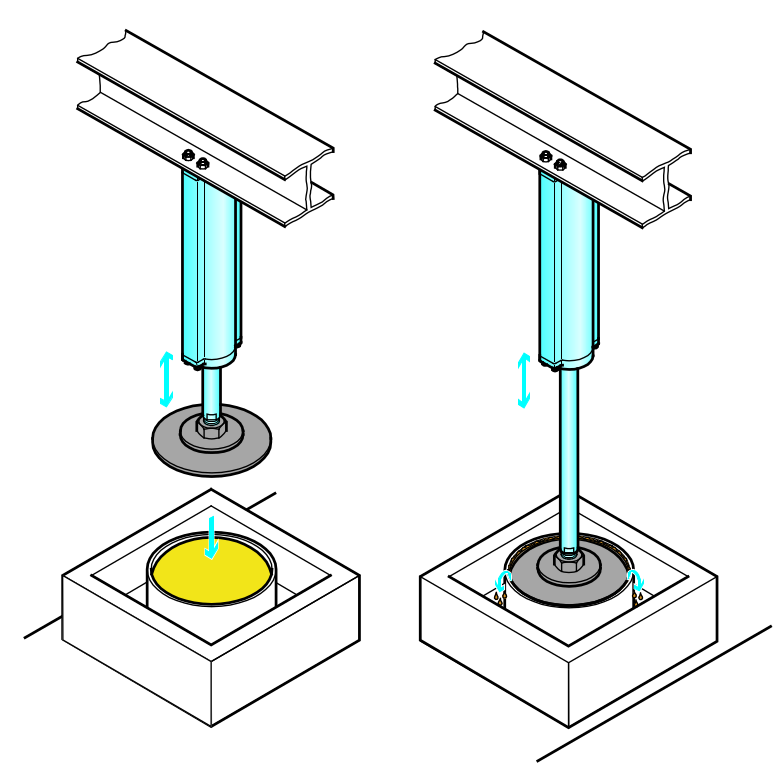
\includegraphics[width=0.5\linewidth]{../../figures/cheese-stamping.png}
\end{center}
{\tiny From FESTO Didactic}
\end{frame}

\begin{frame}[label={sec:org3c71550}]{The Relay}
\begin{center}
\begin{tabular}{cc}
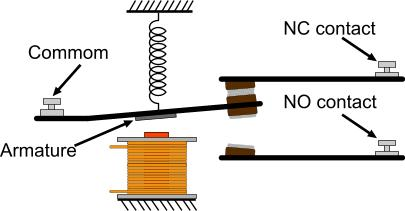
\includegraphics[width=0.4\linewidth]{../../figures/howrelayswork.jpg} &
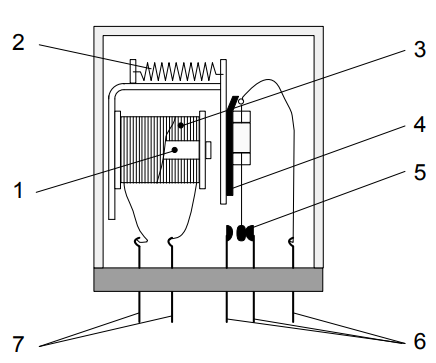
\includegraphics[width=0.3\linewidth]{../../figures/festo-relay-principle.png}\\
{\tiny From pcbheaven.com} & {\tiny From FESTO didactic}\\
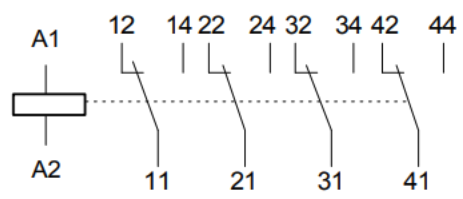
\includegraphics[width=0.35\linewidth]{../../figures/festo-relay-switches.png} &
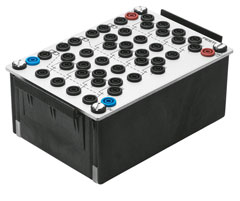
\includegraphics[width=0.25\linewidth]{../../figures/festo-relay-box.jpg}\\
{\tiny From FESTO didactic} & {\tiny From FESTO didactic}\\
\end{tabular}
\end{center}
\end{frame}

\begin{frame}[label={sec:org5344b41}]{Other key components}
{\tiny Sources: FESTO didactic, electroschematics.com, automation-insights.blog}
\begin{columns}
\begin{column}{0.33\columnwidth}
\begin{block}{Limit switch}
\begin{center}
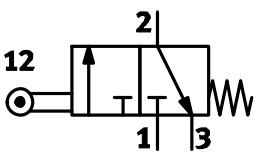
\includegraphics[width=0.4\linewidth]{../../figures/festo-mech-valve-symbol.png}\\
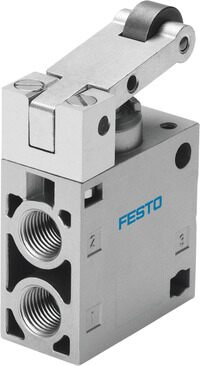
\includegraphics[width=0.3\linewidth]{../../figures/festo-limit-switch.jpg}\\
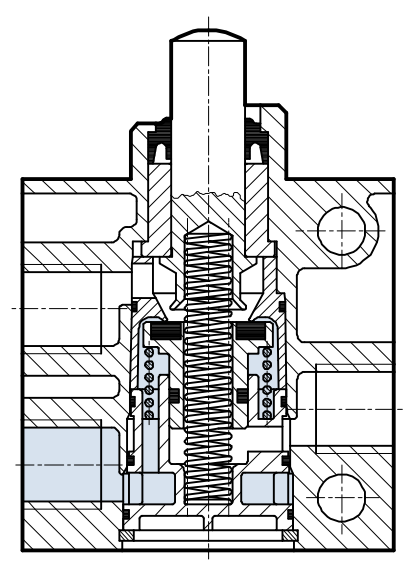
\includegraphics[width=0.5\linewidth]{../../figures/festo-mech-valve-section.png}\\
\end{center}
\end{block}
\end{column}


\begin{column}{0.33\columnwidth}
\begin{block}{Solenoid valve}
\begin{center}
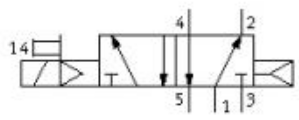
\includegraphics[width=0.7\linewidth]{../../figures/festo-solenoid-52-symbol.png}\\
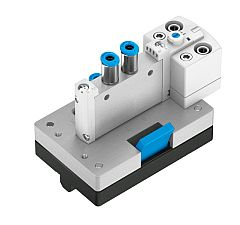
\includegraphics[width=0.45\linewidth]{../../figures/festo-solenoid-52.jpg}\\
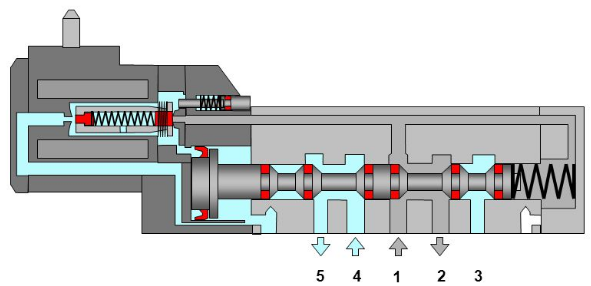
\includegraphics[width=1.1\linewidth]{../../figures/festo-solenoid-schematic.png}\\
\end{center}
\end{block}
\end{column}
\begin{column}{0.33\columnwidth}
\begin{block}{Proximity sensor}
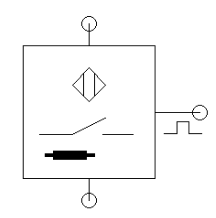
\includegraphics[width=0.4\linewidth]{../../figures/festo-inductive-sensor.png}\\
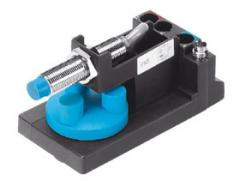
\includegraphics[width=0.6\linewidth]{../../figures/festo-proximity-sensor.jpg}\\
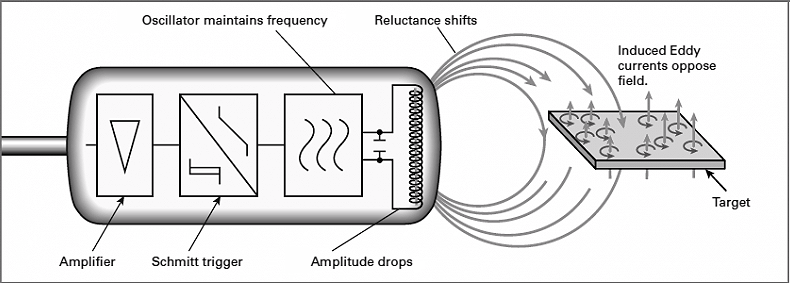
\includegraphics[width=0.99\linewidth]{../../figures/electroschematics-inductive-proximity-sensor.png}\\
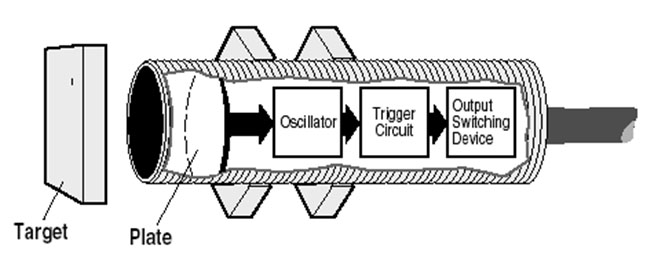
\includegraphics[width=0.99\linewidth]{../../figures/automation-insight-operation_capacitive.jpg}
\end{block}
\end{column}
\end{columns}
\end{frame}


\begin{frame}[label={sec:org8924397}]{A logic control loop}
\begin{center}
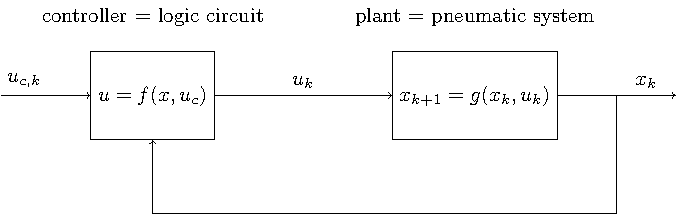
\includegraphics[width=\linewidth]{../../figures/logic-control-loop}
\end{center}
\end{frame}

\begin{frame}[label={sec:org4757311}]{Cheese pressing example - Variables}
\begin{columns}
\begin{column}{0.5\columnwidth}
\begin{block}{State variables}
\(x = \begin{bmatrix} x_R & x_E \end{bmatrix}^T\) with
\begin{align*}
x_R &= \begin{cases} 1 & \text{Cylinder retracted}\\0 & \text{not retracted}\end{cases}\\
x_E &= \begin{cases} 1 & \text{Cylinder extended}\\0 & \text{not extended}\end{cases}
\end{align*}
\end{block}
\begin{block}{Control signal}
\(u = \begin{bmatrix} u_1 & u_2 \end{bmatrix}^T,\) with
\begin{align*}
u_1 &= \begin{cases} 1 & \text{Activate UA+}\\0 & \text{Don't activate UA+ }\end{cases}\\
u_2 &= \begin{cases} 1 & \text{Activate UA-}\\0 & \text{Don't activate UA-}\end{cases}
\end{align*}
\end{block}
\end{column}

\begin{column}{0.5\columnwidth}
    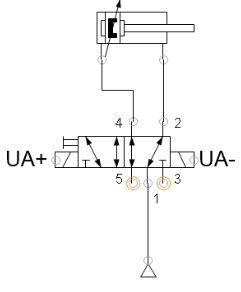
\includegraphics[width=0.6\linewidth]{../../figures/AplAmin-solenoids.png}
Activating solenoid UA+ extends the cylinder, activating  UA- retracts the cylinder.
\begin{block}{Command signal}
\[ u_{c} = \begin{cases} 0 & \text{Button unpushed}\\1 & \text{Button pushed}\end{cases}. \]
\end{block}
\end{column}
\end{columns}
\end{frame}
\begin{frame}[label={sec:org87aef43}]{Cheese pressing example - Plant dynamics}
\begin{block}{Plant dynamics \(x_{k+1} = g(x_k, u_k)\)}
\begin{center}
\begin{tabular}{|cc|cc|cc|}
\hline
Input &  & Current state &  & Next state & \\
\(u_{1,k}\) & \(u_{2,k}\) & \(x_{R,k}\) & \(x_{E, k}\) & \(x_{R,k+1}\) & \(x_{E,k+1}\)\\
 &  &  &  &  & \\
\hline
0 & 0 & 0 & 1 & 0 & 1\\
0 & 1 & 0 & 1 & 1 & 0\\
1 & 0 & 0 & 1 & 0 & 1\\
(1) & (1) & (0) & (1) & (0) & (1)\\
0 & 0 & 1 & 0 & 1 & 0\\
0 & 1 & 1 & 0 & 1 & 0\\
1 & 0 & 1 & 0 & 0 & 1\\
(1) & (1) & (1) & (0) & (1) & (0)\\
\hline
\end{tabular}
\end{center}
\end{block}
\end{frame}


\begin{frame}[label={sec:org32690d2}]{Cheese pressing example - Control law}
The system is operating as long as the start button is pressed (\(u_c=1\)). When the button is released, the cylinder should go to the retracted position.
\begin{block}{Control law \(u_k = f(x, u_c)\)}
\begin{center}
\begin{tabular}{|ccc|cc|}
\hline
\(x_R\) & x\textsubscript{E} & \(u_{c}\) & \(u_1\) & \(u_2\)\\
\hline
0 & 1 & 0 & 0 & 1\\
1 & 0 & 0 & 0 & 0\\
0 & 1 & 1 & 0 & 1\\
1 & 0 & 1 & 1 & 0\\
0 & 0 & 0 & 0 & 1\\
0 & 0 & 1 & 0 & 0\\
\hline
\end{tabular}
\end{center}

\alert{Activity:} Write as boolen functions
\begin{align*}
  u_1 &= f_1(x_R, x_E, u_c) = \qquad\qquad\quad\\
  u_2 &= f_2(x_R, x_E, u_c) =
\end{align*}
\end{block}
\end{frame}
\begin{frame}[label={sec:org19952d1}]{Cheese pressing example - implementing the control  law}
\begin{center}
	 \begin{tikzpicture}
	   \node at (-2,0.5) {+24V};
	   \node at (8,0.5) {0V};
	   \draw (-2,0) to[short, o-]  (-2,-3);
	   \draw (8,0) to[short, o-](8,-3);
	   \draw (6, -0.5) \coil{$u_1$};
	   \draw (6,-2.5) \coil{$u_2$};
      \end{tikzpicture}
\end{center}
\begin{center}
  \begin{tikzpicture}
    \draw(0,0) to [push button, label={normally open}] ++(2,0);
    \draw(5,0) to [pushed button, label={normally closed}] ++(2,0);
  \end{tikzpicture}
\end{center}
\begin{center}
  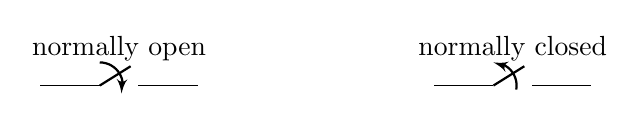
\begin{tikzpicture}
    \draw(0,0) to [switch, label={normally open}] ++(2,0);
    \draw(5,0) to [opening switch, label={normally closed}] ++(2,0);
  \end{tikzpicture}
\end{center}
\begin{center}
  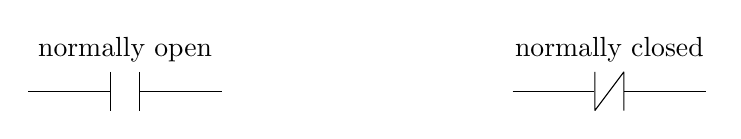
\begin{tikzpicture}[circuit plc ladder,]
    \draw(0,0) to [contact NO={info={normally open}}] ++(2,0);
    \draw(5,0) to [contact NC={info={normally closed}}] ++(2,0);
  \end{tikzpicture}
\end{center}
\end{frame}

\section{Latching circuit}
\label{sec:orgad529d2}
\begin{frame}[label={sec:org32dccef}]{An electrical circuit with memory}
\begin{center}
\begin{tabular}{cc}
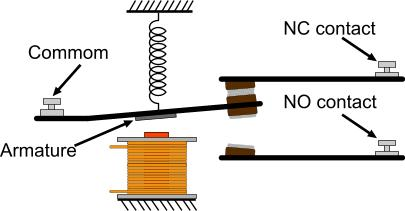
\includegraphics[width=0.4\linewidth]{../../figures/howrelayswork.jpg} &
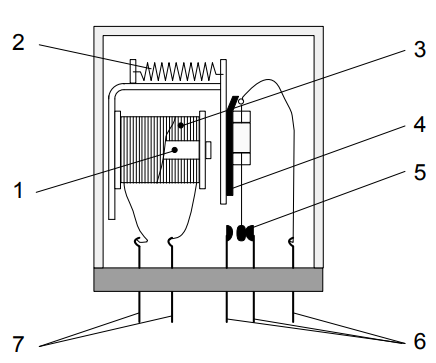
\includegraphics[width=0.3\linewidth]{../../figures/festo-relay-principle.png}\\
{\tiny From pcbheaven.com} & {\tiny From FESTO didactic}\\
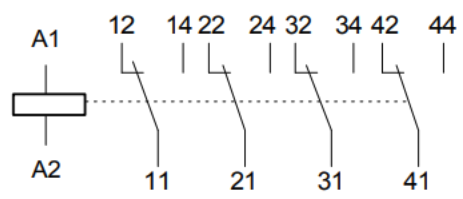
\includegraphics[width=0.35\linewidth]{../../figures/festo-relay-switches.png} &
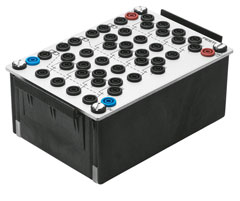
\includegraphics[width=0.25\linewidth]{../../figures/festo-relay-box.jpg}\\
{\tiny From FESTO didactic} & {\tiny From FESTO didactic}\\
\end{tabular}
\end{center}
\end{frame}

\begin{frame}[label={sec:orge1508de}]{An electrical circuit with memory}
\begin{columns}
\begin{column}{0.6\columnwidth}
\begin{block}{Latching circuit}
\begin{center}
         \begin{tikzpicture}
           \node at (0,0.5) {+24V};
           \node at (6,0.5) {0V};
           \draw (0,0) to[short, o-]  (0,-2.5);
           \draw (6,0) to[short, o-](6,-2.5);
           \draw (0,-0.3) to[push button, label={$X$}] (2,-0.3) to[pushed button, label=$Y$, ] (4,-0.3) to[short] (4,-0.3) to[twoport, label={$R$}] (6,-0.3); %\coil{$R$};
           \draw (0,-2) to[switch,label={$R$}] (2,-2)  to[short] (2,-0.3);
         \end{tikzpicture}
\end{center}
\begin{center}
         \begin{tikzpicture}[circuit plc ladder,]
           \node at (0,0.5) {+24V};
           \node at (6,0.5) {0V};
           \draw (0,0) to[short, o-]  (0,-2.5);
           \draw (6,0) to[short, o-](6,-2.5);
           \draw (0,-0.3) to[contact NO={info={$X$}},] (2,-0.3) to[ contact NC={info={$Y$}}, ] (4,-0.3) to[short] (4,-0.3) \coil{$R$};
           \draw (0,-2) to[contact NO={info={$R$}},] (2,-2)  to[short,] (2,-0.3);
         \end{tikzpicture}
\end{center}
\end{block}
\end{column}


\begin{column}{0.4\columnwidth}
\begin{block}{Truth table}
\begin{center}
\begin{tabular}{|ccc|c|}
\(X\) & \(Y\) & \(R_k\) & \(R_{k+1}\)\\
\hline
0 & 0 & 0 & \\
0 & 0 & 1 & \\
0 & 1 & 0 & \\
0 & 1 & 1 & \\
1 & 0 & 0 & \\
1 & 0 & 1 & \\
1 & 1 & 0 & \\
1 & 1 & 1 & \\
\hline
\end{tabular}
\end{center}

\alert{Group activity:} Implement the circuit in FluidSim and verify the truth table.
\end{block}
\end{column}
\end{columns}
\end{frame}
\end{document}